Habiendo definido nuestros algoritmos, lo que nos queda es ver cuál es la ventaja que otorgan los mismos en comparación a la solución naive de cada uno de estos problemas. Esta ventaja puede ser en precisión, tiempo o espacio. 

Para los experimentos utilizamos dos redes bayesianas, $\cancerNetwork$ y $\childNetwork$ tomadas del paquete de R \href{https://www.bnlearn.com/bnrepository/}{bnlearn}, podemos ver su estructura en la Figura \ref{fig:bayesian_networks_combined}. Utilizamos estas redes, ya que tenían un tamaño manejable y una topología similar a la de un polytree. Además de ser la distribución de nuestros datos, las empleamos cómo nuestros grafos causales, asumiendo que fueron generadas basándose en la causalidad \footnote{Esto no necesariamente siempre se cumple, pero entendemos que es una suposición razonable para la mayoría de los casos.}.
 En el caso de la red \childNetwork, al no ser un polytree tuvimos que remover algunas aristas para lograr obtener esa estructura. Analizamos distintas heurísticas para remover ejes de la red, para convertirla en un polytree, utilizamos la más sencilla que consiste en remover los ejes que generan ciclos en el grafo subyacente de la red bayesiana. Una opción más refinada consiste en elegir las aristas a remover, minimizando la divergencia entre las distribuciones marginalizadas. Esto lo podríamos hacer comparando las distintas distribuciones que nos quedan al remover distintas aristas, utilizando una métrica como la divergencia de Kullback-Leibler, pero no era el objetivo de esta tesis. 

Para generar los datasets de entrenamiento y test, sampleamos instancias de ambas redes. Luego entrenamos al DT usando este dataset. A la hora de calcular el ASV, removimos la variable a predecir de nuestra red. Removemos la variable, puesto que si tuviéramos la red bayesiana completa con nuestra variable a predecir en la misma, haríamos la inferencia directamente en la red bayesiana \footnote{Tampoco entrenaríamos un árbol de decisión, sino que simplemente utilizaríamos a la red para clasificar las instancias}. Las variables que definimos para predecir fueron \variableNetwork{Smoker} y \variableNetwork{Age} para sus respectivas redes. En el caso de la red $\cancerNetwork$ no elegimos \variableNetwork{Cancer}, puesto que nuestro DAG causal iba a perder todas sus dependencias, por lo cual ASV no iba a poder detectar relaciones significativas. Luego en el caso de \childNetwork{} el criterio fue no utilizar una variable que se encuentre muy arriba en el árbol, puesto que no iba a tener muchas variables que la influencien, ni tan abajo que cueste distinguir las variables que la impactan mayormente. Por lo que nuestro input va a ser una red bayesiana $\aBayesianNetwork$, un feature a predecir $p$, un dataset $data$, un árbol de decisión $DT$ y una instancia $x \in data$. 

\begin{figure}[ht]
    \centering

    \begin{subfigure}[b]{0.3\textwidth}
        \centering
        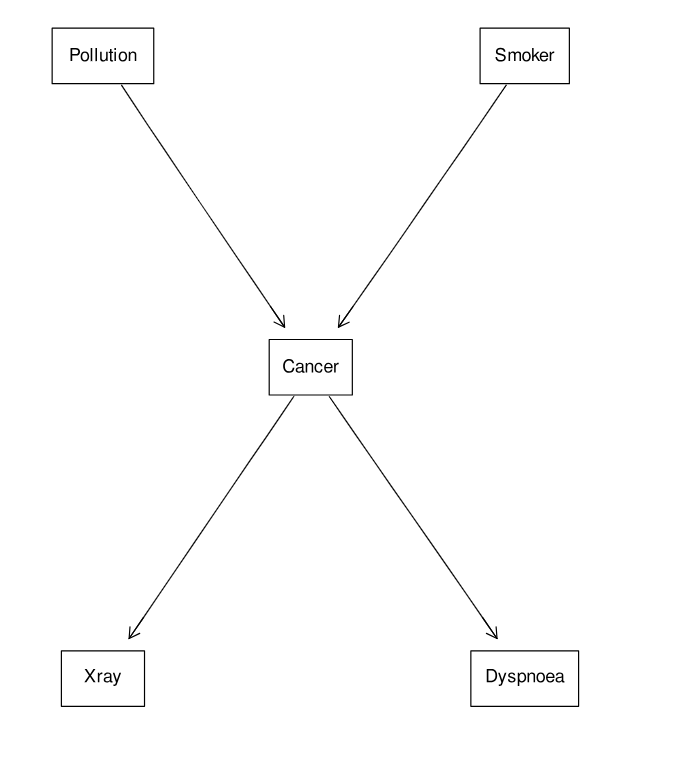
\includegraphics[width=\textwidth]{img/bayesianNetworks/cancerNetwork.png}
        \caption{Red Bayesiana $\childNetwork$ para analizar las enfermedades de niños de recién nacidos. Fuente: \cite{cancerNetwork}}
        \label{fig:cancer_network}
    \end{subfigure}
    \hfill
    \begin{subfigure}[b]{0.6\textwidth}
        \centering
        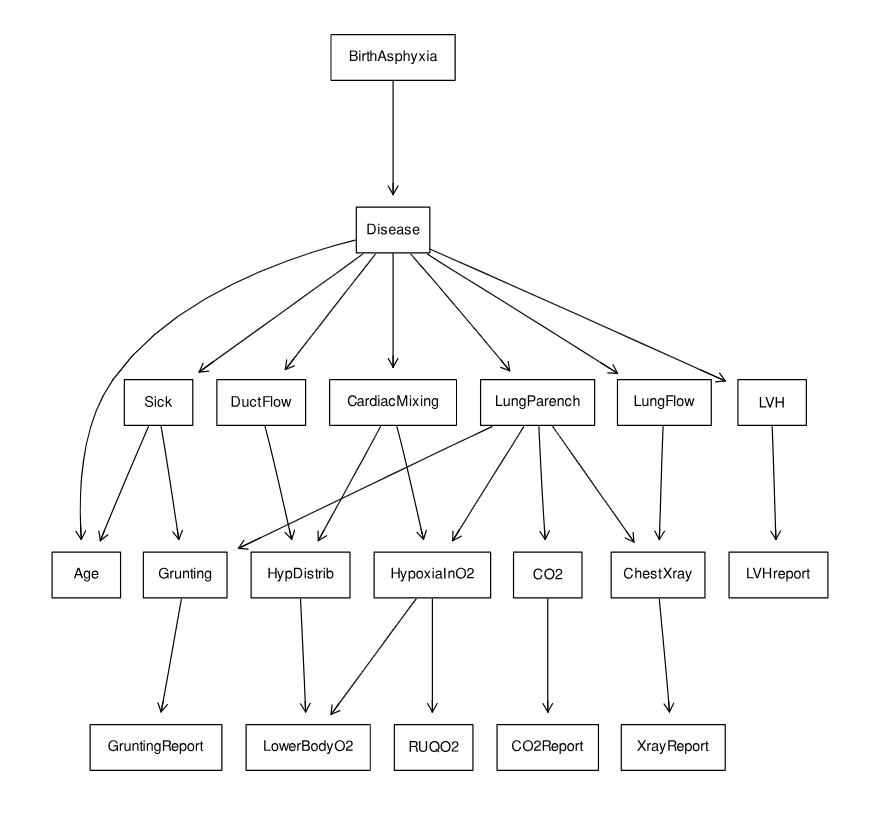
\includegraphics[width=\textwidth]{img/bayesianNetworks/childNetwork.png}
        \caption{Red Bayesiana para determinar la probabilidad de tener cáncer de distintos pacientes. Fuente: \cite{childNetwork}}
        \label{fig:child_network}
    \end{subfigure}

    \caption{Ejemplos de redes bayesianas utilizadas en los experimentos.}
    \label{fig:bayesian_networks_combined}
\end{figure}

\paragraph{Especificaciones de los experimentos}

\begin{itemize}
    \item \textbf{Procesador:} Intel(R) Core(TM) i5-7500 CPU @ 3.40GHz
    \item \textbf{Memoria RAM:} 16 GB
    \item \textbf{Sistema operativo:} Ubuntu 22.04 LTS
    \item \textbf{Python:} Versión 3.12
    \item  \textbf{Paquetes:} pgmpy (inferencia bayesiana), sklearn, networkx, shap
\end{itemize}

\subsection{Clases de equivalencia vs Órdenes Topológicos}

Para este experimento, vamos a comparar la implementación clásica de $ASV$ con nuestra idea de utilizar las clases de equivalencia para reducir los términos de la sumatoria. Para eso vamos a comparar la forma original de calcular ASV: 

$$\frac{1}{|topos(G)|} \sum_{\pi \in topos(G)} w(\pi) \left[ \charactheristicFunction(\pi_{<i} \cup {i}) - \charactheristicFunction(\pi_{<i}) \right] $$
con nuestra heurística:
$$\heuristicASVFormula$$

Hay dos métricas a tener en cuenta para ver cual de estas dos estrategias es mejor. Primero, ver cuánto es el tiempo que se tarda en obtener los conjuntos sobre los que efectuar la sumatoria, que son $eqCl(G, x_i)$ y $topos(G)$. Luego comparar el tamaño de cada uno de esos conjuntos, puesto que por cada elemento de ese conjunto vamos a tener que evaluar a $\charactheristicFunction$ dos veces. Podría ocurrir que la construcción de las clases de equivalencia resulte computacionalmente costosa, y su cardinalidad no necesariamente presente una reducción significativa en comparación con $topos$. En tales casos, el costo adicional de calcularlas puede superar el beneficio esperado, incrementando el tiempo total de cómputo.

\begin{figure}[ht]
    \centering
    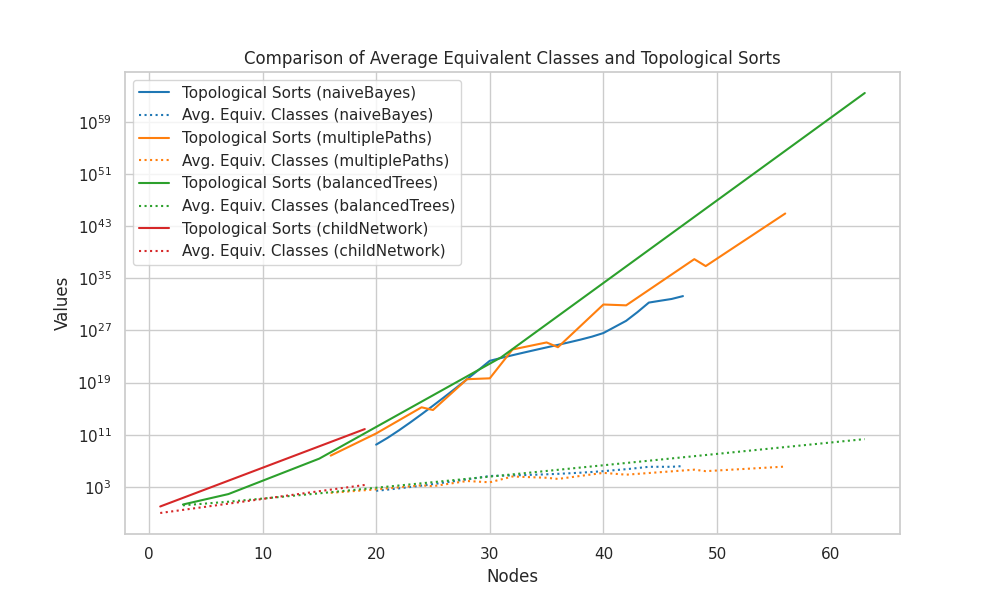
\includegraphics[width=1\linewidth]{img/equivalentClassesVsToposorts.png}
     \caption[Caption for image]{Comparación de clases de equivalencias y órdenes topológicos de distintas clases de grafos. Se utiliza un promedio, puesto que la cantidad de clases de equivalencia depende del nodo que elijamos para calcularlas. \footnotemark }
    \label{fig:equivalenceClassesVsToposortsNumberPlot}
\end{figure}

\footnotetext{La función no es monótona ya que no se utilizaron todos los grafos posibles para cada una de las clases mencionadas, se realizó una estimación a partir de una muestra significativa de distintos grafos de cada clase. }

%\echu{¿Es mejor tener un gráfico para cada familia? A mi me parecía mejor unificarlos} Queda unificado

Las distintas clases de grafos mencionados en la Figura \ref{fig:equivalenceClassesVsToposortsNumberPlot} son: 
\begin{itemize}
    \item Naive Bayes: Una red Naive Bayes con $n$ nodos, que tiene $n/2$ hojas y que tiene un camino de longitud $n/2-1$ en una de sus hojas. %\santi{No dan las cuentas de la cantidad de nodos} \echu{¿Ahí si, no? Me faltaba la raíz}
    \item Multiple paths: Un bosque compuesto de múltiples caminos de igual longitud. 
    \item Balanced tree: Un árbol binario perfecto balanceado.  
    \item Child network: La red bayesiana \childNetwork, sin algunos de sus ejes para ser un polytree. 
    
\end{itemize}

En la Figura \ref{fig:equivalenceClassesVsToposortsNumberPlot}, podemos observar como el número de clases de equivalencia crece significativamente más lento que el número de órdenes topológicos. Por ejemplo, en el caso de la red $\childNetwork$, la red tiene $7.41\times10^{11}$ órdenes topológicos y 2003 clases de equivalencia en promedio, por lo que si utilizamos las clases disminuimos enormemente la cantidad de llamadas a $\charactheristicFunction$. Luego, para los árboles balanceados, la cantidad de órdenes topológicos es $10^{50}$ veces mayor, una diferencia muy significativa. A partir de estos ejemplos, queda claro que es una mejora hacer el cálculo sobre las clases de equivalencia, ahora sólo queda ver el costo de calcularlas. 

El costo de calcular las clases lo podemos ver en la Figura \ref{fig:equivalenceClassesTimePlot}, para la mayoría de los grafos de ejemplo que utilizamos tarda menos de 10 segundos. Pero para grafos de mayor tamaño, el tiempo que tarda comienza a crecer exponencialmente, al igual que la cantidad de clases de equivalencia. En el caso puntual de la red \childNetwork, tarda menos de 1 segundo en calcular todas sus clases. 


\begin{figure}[ht]
    \centering
    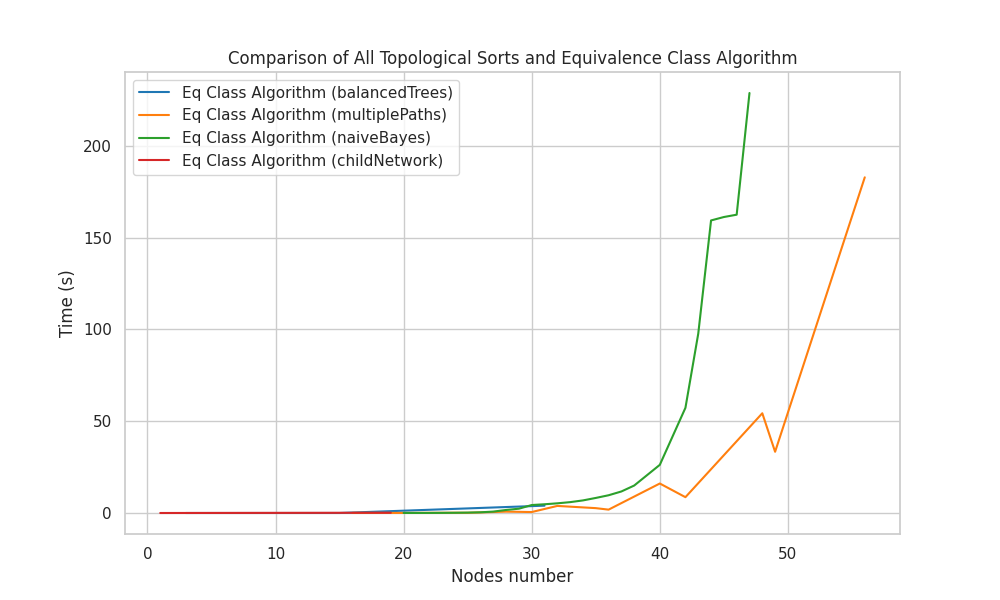
\includegraphics[width=1\linewidth]{img/equivalentClasses_time.png}
    \caption[Caption for image]{Comparación del tiempo que tarda el algoritmo para calcular las clases de equivalencia}
    \label{fig:equivalenceClassesTimePlot}
\end{figure}

\begin{figure}[ht]
    \centering
    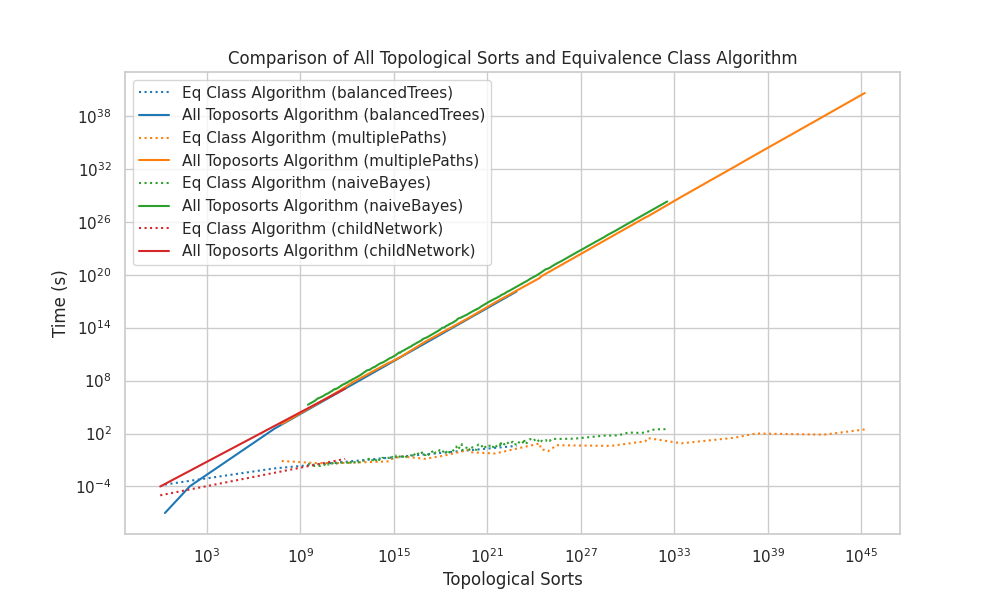
\includegraphics[width=1\linewidth]{img/equivalentClassesVsAllToposorts_time.png}
    \caption[Caption for image]{Comparación del tiempo que tarda el algoritmo para calcular las clases de equivalencia y calcular todos los órdenes topológicos, utilizando una \href{https://networkx.org/documentation/stable/reference/algorithms/generated/networkx.algorithms.dag.all_topological_sorts.html}{implementación} de la librería networkx. \footnotemark }
    \label{fig:equivalenceClassesVsToposortsTimePlot}
\end{figure}


\footnotetext{Para estimar el tiempo que tardaría se calcularon los primeros 1000 órdenes que devuelve el algoritmo exacto. Luego se utilizó ese tiempo para hacer una aproximación del tiempo total, sabiendo la cantidad de órdenes de cada grafo. Esto se realizó por simplicidad ya que no era viable correr el algoritmo durante tanto tiempo.}

La Figura \ref{fig:equivalenceClassesVsToposortsTimePlot} nos muestra para distintos tipos de grafos cuánto tiempo toma cada algoritmo. En uno se obtienen todas las clases de equivalencia y en el otro todos los órdenes topológicos. A partir de $10^{15}$ órdenes topológicos el problema de calcularlos todos tardaría días, en cambio, calcular las clases de equivalencia sigue siendo una estrategia eficiente. Esto sucede así, puesto que, como vimos en el lema \ref{lemma:upper_bound_equivalence_classes}, la cantidad de clases de equivalencia depende de la estructura del grafo, y no de la cantidad de órdenes.
%\sergio{revisar esta frase, no tiene sentido que solo a partir de $10^{15}$ no es tratable} Rta: Ahí le puse la referencia al gráfico correspondiente y tuvo más sentido, si no era cualquier cosa. 

Por ende, a través de este experimento pudimos ver que la cantidad de clases de equivalencias es significativamente menor que la cantidad de órdenes, por lo que se reduce la cantidad de llamadas a $\charactheristicFunction$. Además, en la figura \ref{fig:equivalenceClassesVsToposortsTimePlot}, podemos ver cómo crece más lentamente el tiempo para calcular las clases de equivalencia, que el tiempo de calcular todos los órdenes. Por lo que el algoritmo proporciona una mejora, respecto a la implementación naive, del tiempo para calcular todas las clases.
%\echu{Medio raro lo de doblemente efectiva, tal vez habría que expresarlo de otra forma}
%\sergio{Decir algo de que cambia el slope en la escala logarítmica notablemente}

\subsection{ASV vs SHAP}

%\echu{¿Uso emph, bold o alguna otra notación para las redes y las variables?} Sip, emph para redes y texttt para las variables

Este experimento consiste en calcular el valor del $ASV$ y $SHAP$, para cada uno de los features de los modelos utilizados en el experimento de la sección \ref{subSection:experimentoAlgoritmoPromedio}. Vamos a correr este experimento para 5 seeds distintas, ya que los valores obtenidos pueden depender de la aleatoriedad de los datos y queremos contrastar múltiples resultados. Aun así, vamos a elegir una seed para analizar para cada una de las redes, utilizando como criterio para elegir la seed el modelo con la mejor accuracy, ya que si el modelo no aprendió correctamente los patrones subyacentes de los datos, entonces los valores de $ASV$ y $SHAP$ pueden no correlacionarse con el grafo causal original. Los resultados de todas las corridas pueden verse en el apéndice en las Figuras ~\ref{fig:multipleSeedsASVvsShapleyChild} y \ref{fig:multipleSeedsASVvsShapleyCancer}. Correr el $ASV$ para todos los features de la red $\cancerNetwork$ tarda 1 segundo, y correrlo para todos los features de la red $\childNetwork$ tarda 3 minutos. 

Para obtener una intuición acerca de ambas redes y las distintas relaciones entre sus nodos nos basamos en \cite{childNetwork} para la red $\childNetwork$ y \cite{cancerNetwork} para la red $\cancerNetwork$. Además generamos una Tabla \ref{tab:phi_smoker_with_shift} para ambas redes, para analizar el impacto de modificar cada una de las variables de la red. Por ejemplo, la probabilidad original de la variable \variableNetwork{Smoker} es $P(Smoker=True)=0.3$ pero si sabemos que el paciente tiene cáncer pasa a ser $P(Smoker=True|Cancer=True)=0.8255$. Por lo que (como era de esperarse), \variableNetwork{Cancer} es una variable significativa a la hora de calcular si un paciente es fumador o no. En este caso, vemos que la probabilidad de que sea fumador se vio modificada en 0.5255 al introducir la evidencia de que tenía \variableNetwork{Cancer}. Esta variación de la probabilidad es la que vamos a ver en la columna \emph{Probability Shift} en la Tabla \ref{tab:phi_smoker_with_shift}.

\begin{table}[ht]
    \centering
    \begin{tabular}{|c|c|c|c|}
        \hline
        \textbf{Variable} & \textbf{Smoker} & \textbf{New smoker probability} & \textbf{Probability Shift} \\
        \hline
        \multirow{2}{*}{Pollution = Low} & True  & 0.3 & \multirow{2}{*}{0.0} \\
                                         & False & 0.7 & \\
        \hline
        \multirow{2}{*}{Pollution = High} & True  & 0.3 & \multirow{2}{*}{0.0} \\
                                          & False & 0.7 & \\
        \hline
        \multirow{2}{*}{Cancer = True} & True  & 0.8255 & \multirow{2}{*}{0.5255} \\
                                       & False & 0.1745 & \\
        \hline
        \multirow{2}{*}{Cancer = False} & True  & 0.2938 & \multirow{2}{*}{0.0062} \\
                                        & False & 0.7062 & \\
        \hline
        \multirow{2}{*}{Xray = Positive} & True  & 0.3206 & \multirow{2}{*}{0.0206} \\
                                         & False & 0.6794 & \\
        \hline
        \multirow{2}{*}{Xray = Negative} & True  & 0.2946 & \multirow{2}{*}{0.0054} \\
                                         & False & 0.7054 & \\
        \hline
        \multirow{2}{*}{Dyspnoea = True} & True  & 0.3070 & \multirow{2}{*}{0.0070} \\
                                         & False & 0.6930 & \\
        \hline
        \multirow{2}{*}{Dyspnoea = False} & True  & 0.2969 & \multirow{2}{*}{0.0031} \\
                                          & False & 0.7031 & \\
        \hline
    \end{tabular}
    \caption{Variación de la probabilidad de ser fumador en base a la nueva evidencia}
    \label{tab:phi_smoker_with_shift}
\end{table}

Comencemos analizando el caso de la red $\cancerNetwork$. En la Figura \ref{fig:shapleyVsASVSingleSeedCancer} podemos ver que para $ASV$ la única variable significativa es \variableNetwork{Cancer}. Esto tiene sentido con lo visto en la Figura \ref{fig:cancer_network}, ya que es la única variable conectada directamente con \variableNetwork{Smoker}. Pero si nos basáramos en los resultados obtenidos en los Shapley Values, creeríamos que \variableNetwork{Xray} y \variableNetwork{Dyspnoea} también tienen un impacto significativo en si es fumador o no el paciente. La forma que tenemos para ver cuál de los métodos está detectando correctamente las variables relevantes es la Tabla \ref{tab:phi_smoker_with_shift}, en la cual podemos ver que la variable que más impacta es \variableNetwork{Cancer} y que la \variableNetwork{Dyspnoea} tiene un impacto mucho menor. Esta nueva métrica que vamos a utilizar, es igual de arbitraria que Shap, pero nos permitió realizar una comparación y un análisis cuantitativo más allá del significado de cada una de las variables 
%\santi{Nunca definís como se calcula el probability shift}
%\echu{Esto quedo medio raro, lo que quiero decir es que utilizamos esta métrica para que la justificación meramente no sea "Tiene sentido esto, por lo que significan las variables en el mundo real" ¿Se entiende la idea?}.
%\santi{Se entiende, creo.}
Esto ocurre ya que $ASV$ tiene en cuenta el grafo causal a la hora de realizar estos cálculos, a diferencia de $SHAP$. 

\begin{figure}
    \centering
    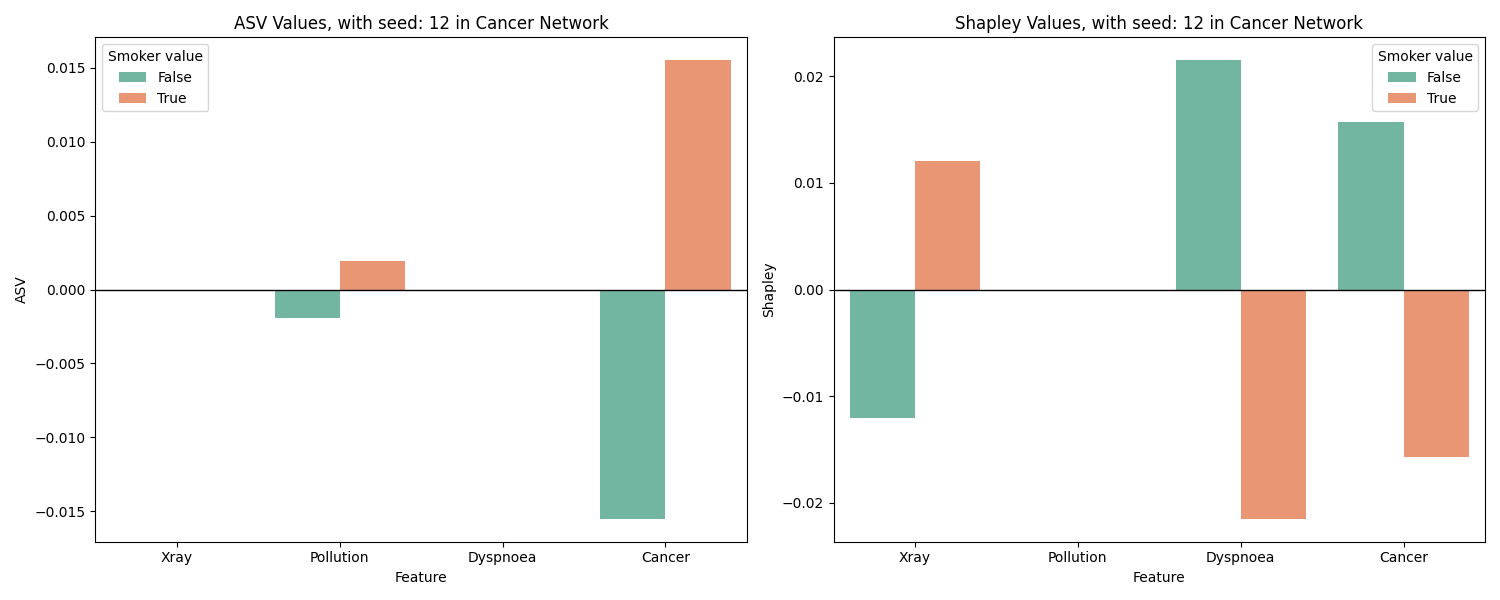
\includegraphics[width=1\linewidth]{img/asvResults/cancerASVAndShapleyExactASVAndShapley.png}
    \caption{Resultados del ASV y Shapley para el modelo con mayor accuracy de los 5 seeds para la red $\cancerNetwork$, con un 81\% de accuracy. }
    \label{fig:shapleyVsASVSingleSeedCancer}
\end{figure}

Luego en el caso de la red $\childNetwork$, estas son las 5 variables más relevantes para las distintas métricas propuestas:

\begin{itemize}
    \item \textbf{Mayor valor de Probability Shift}: Disease, Duct Flow, Sick, Cardiac Mixing, LVH
    \item \textbf{Mayor valor de ASV}: Disease, Duct Flow, Sick, LVH, LVH Report
    \item \textbf{Mayor valor de SHAP}: Disease, ChestXRay, CO2, RUQO2, LVH Report
\end{itemize}

Estos resultados\footnote{Los datos completos se pueden encontrar en \path{\pasantia-BICC\results}, para ver la tabla completa para todas las variables.} se basan en la Figura \ref{fig:shapleyVsASVSingleSeedChild}. Lo que podemos ver es que la intersección entre los features más relevantes de Probability Shift y $ASV$, es mayor a la de $SHAP$ con la misma métrica. Ya que aunque ambos logran identificar a los nodos \variableNetwork{Disease} y a \variableNetwork{LVH/LVH Report} como relevantes, sólo $ASV$ encuentra la relación con \variableNetwork{Sick} y \variableNetwork{DuctFlow}. Aún así esto podría variar según el modelo, ya que si el modelo no logró identificar correctamente las relaciones entre los datos, los valores de $ASV$ y $SHAP$ tampoco van a correlacionarse con el grafo causal. Analizar estos valores, nos puede ayudar a ver si tiene sentido la elección de features más relevantes que está utilizando nuestro algoritmo para realizar sus predicciones. 
%\echu{Acá lo polémico es que uso la nueva métrica, Probability Shift, cómo un tipo de ground truth para ver cuáles son los features más relevantes}
%\santi{Si, se ve la complicación. Capaz estaría bueno decir algo más o comparar con otras métricas, pero buneo. Creo igual que el primer ejemplo ya convence de que hay algo raro en SHAP.} Rta: Lo dejamos así también, es lo polémico de usar métricas para comparar. Ninguna es mejor que todas

\begin{figure}
    \centering
    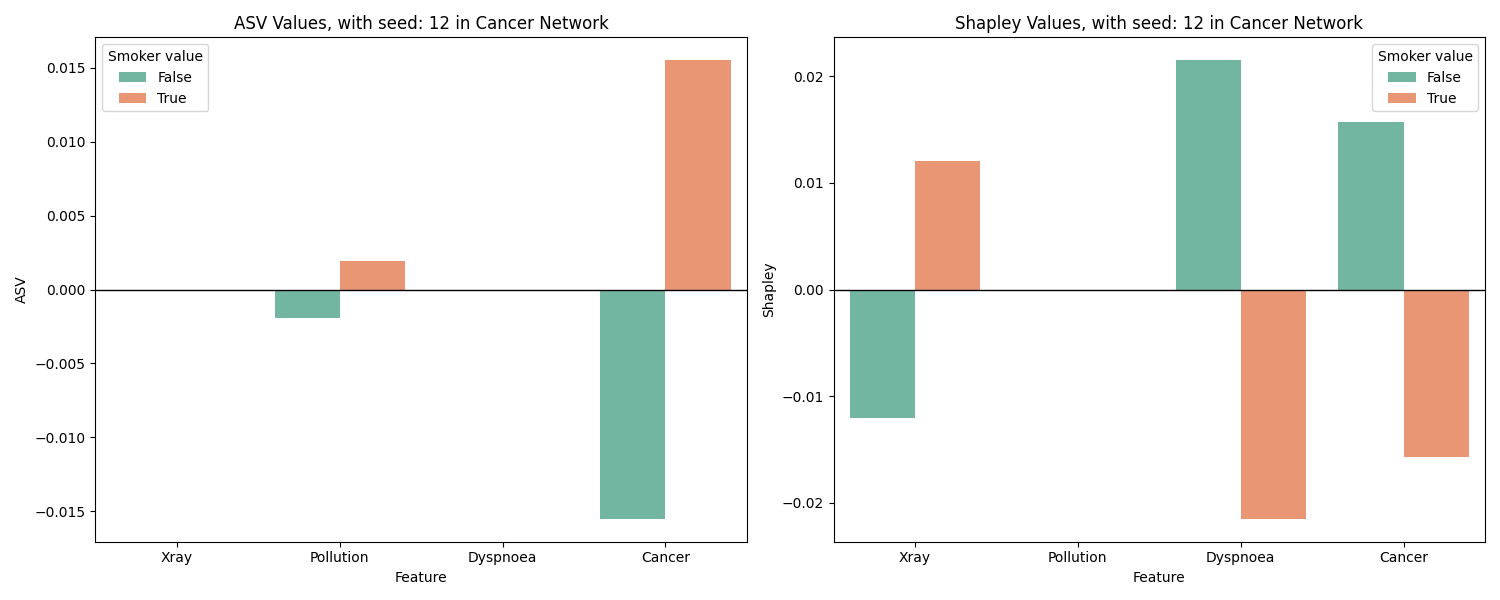
\includegraphics[width=1\linewidth]{img/asvResults/cancerASVAndShapleyExactASVAndShapley.png}
    \caption{Resultados del ASV y Shapley para el modelo con mayor accuracy de los 5 seeds para la red $\childNetwork$, con un 68\% de accuracy. }
    \label{fig:shapleyVsASVSingleSeedChild}
\end{figure}

En base a lo observado en estos dos casos, podemos ver que $ASV$ puede detectar relaciones entre los features que $SHAP$ no logra encontrar. Esto se debe a que utiliza la información del grafo causal, para ver cuales features priorizar a la hora de realizar estos cálculos. 

\subsection{ASV exacto sin EqClasses vs ASV aproximado}

El objetivo de este experimento es comparar la performance de obtener los órdenes topológicos de un grafo que es un polytree, pero no es un \dtree. Por lo tanto sólo los podemos obtener sampleandolos con nuestro Algoritmo \ref{alg:topoSortSampling} o generándolos con el algoritmo de Knuth, puesto que las clases de equivalencia sólo las podemos obtener para los \dtrees.

\begin{table}[h]
\centering
\begin{tabular}{|l|c|}
\hline
\textbf{Cantidad de órdenes sampleados} & \textbf{Tiempo de sampleo (s)}\\
    \hline
    100 & 0.9270 \\
    1000 & 1.1170 \\
    10000 & 4.7170 \\
    20000 & 7.7170 \\
    30000 & 10.8387 \\
    \hline
    \end{tabular}

\caption{Tiempos de ejecución para muestreo y generación de órdenes topológicos de la red $\childNetwork$}
\label{table:exactVsApproximateTopoSorts}
\end{table}

En la Tabla \ref{table:exactVsApproximateTopoSorts} podemos ver que el enfoque aproximado toma un tiempo tratable para samplear los órdenes. Aunque en nuestro análisis de la complejidad del mismo, habíamos llegado a una cota cuasi polinomial, el algoritmo se comporta de mejor manera en la práctica. También podemos observar que, cómo se mencionó al introducir el algoritmo de sampleo, su complejidad no es lineal en la cantidad de órdenes sampleados. Esto ocurre, pues vamos obteniendo múltiples candidatos en cada llamado recursivo de la función. 

En base a estos resultados, uno podría creer que la mejor opción es generarlos con el algoritmo de Knuth, el cuál tarda menos de 1 segundo en generar los 30000 órdenes. El problema de este algoritmo es que no respeta la distribución de los órdenes.  Por ejemplo, si tuviéramos un grafo como el de la Figura \ref{fig:badExactToposortExample}, podría ocurrir que los primeros 1000 órdenes que nos devuelva el algoritmo tengan como primer nodo a $n_1$. Pero en realidad $n_1$ es el primer nodo en menos del 0.05\% de los casos. Por lo que no sería una muestra representativa. Para lograr esto deberíamos generar todos los órdenes, pero ya generar meramente un 1\% de los órdenes de la red $\childNetwork$ tomaría más de 2 días. 

%\echu{Este ejemplo, no tan detallado, lo mencionó también en el segundo parrafo de la sección de sampleo. ¿Vale la pena este experimento? Para mi esta bueno para ilustrar porque no garpa usar el algoritmo de Knuth, aunque no sume tantooo}

%\santi{Me parece bien.}

\begin{figure}[ht]
    \centering
    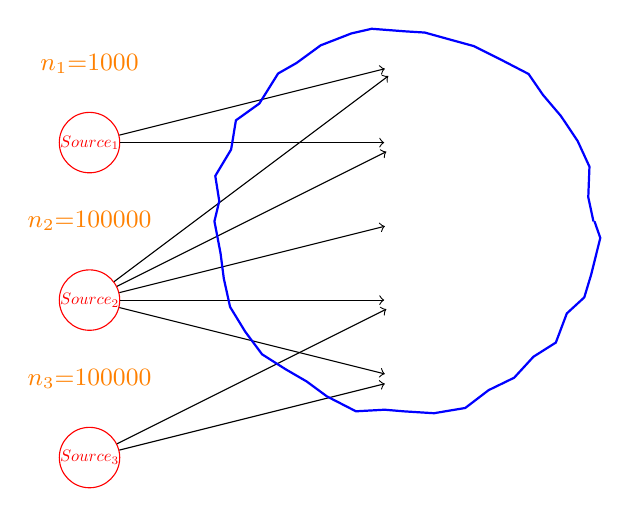
\begin{tikzpicture}
        % Define the rigth set of nodes
        \foreach \i in {1,2,3,4,5}
            \node[draw=none, circle, minimum size=5mm, inner sep=0pt] (L\i) at (4, -\i) {};

        % Define the left set of nodes
        \foreach \j in {1,2,3}
            \node[draw, circle, red, minimum size=5mm, inner sep=0pt] (source\j) at (0, -\j*2) {\scalebox{0.6}{$Source_\j$}};

        % Draw edges between nodes (example edges)
        \foreach \i in {1,2}
            \foreach \j in {1,2}
                \draw[->]  (source\j) -- (L\i); 

        \foreach \i in {4,5}
            \foreach \j in {2,3}
                \draw[->]  (source\j) -- (L\i); 

        \draw[->]  (source2) -- (L3);
        

         \draw [decorate, blue, decoration={random steps, segment length=10pt, amplitude=2pt}, thick]
        (4,-3) circle (2.4);

        %Número de ordenes topológicos para cada nodo

        \node[draw=none,minimum size=3mm, inner sep=0pt] () at (0, -1) {\small \textcolor{orange}{$n_1$=1000}};

        \node[draw=none,minimum size=3mm, inner sep=0pt] () at (0, -3) {\small \textcolor{orange}{$n_2$=100000}};

        \node[draw=none,minimum size=3mm, inner sep=0pt] () at (0, -5) {\small \textcolor{orange}{$n_3$=100000}};
    \end{tikzpicture}
    \caption{Posible comienzo del algoritmo exacto. Con los candidatos a ser el primer nodo del orden en rojo y el resto del grafo en azul. Cada node fuente (source) tiene sus respectivas cantidades de órdenes topológicos en los que está primero.}
    \label{fig:badExactToposortExample}
\end{figure}

Por último realizamos un experimento para calcular el error al calcular $ASV$ con el método aproximado, sampleando 1000 ordenes topológicos de la red $\childNetwork$. En la Figura \ref{fig:boxplotASVApproximateDifferences} podemos ver los resultados de esta corrida. La mayoría de los valores aproximados obtenidos tiene un error del 8\% con respecto a su valor exacto. Las diferencias más altas se corresponden a valores de $ASV$ muy pequeños, como 0.005, por lo que una pequeña diferencia en su valor calculado relativamente es más significativa. Esto es esperable, ya que el error mencionado en el Teorema \ref{theorem:asvSamplingError} es un error absoluto, no relativo. Para los features con valores mayores a 0.01, su diferencia es menor al 5\%.
%\santi{Esto es esperable: nuestro teorema habla de error absoluto, no del relativo. Podrías decirlo.}
Con estos resultados, podemos concluir que no es necesario obtener todos los ordenes y con una buena aproximación podemos obtener resultados medianamente precisos. 


\begin{figure}
    \centering
    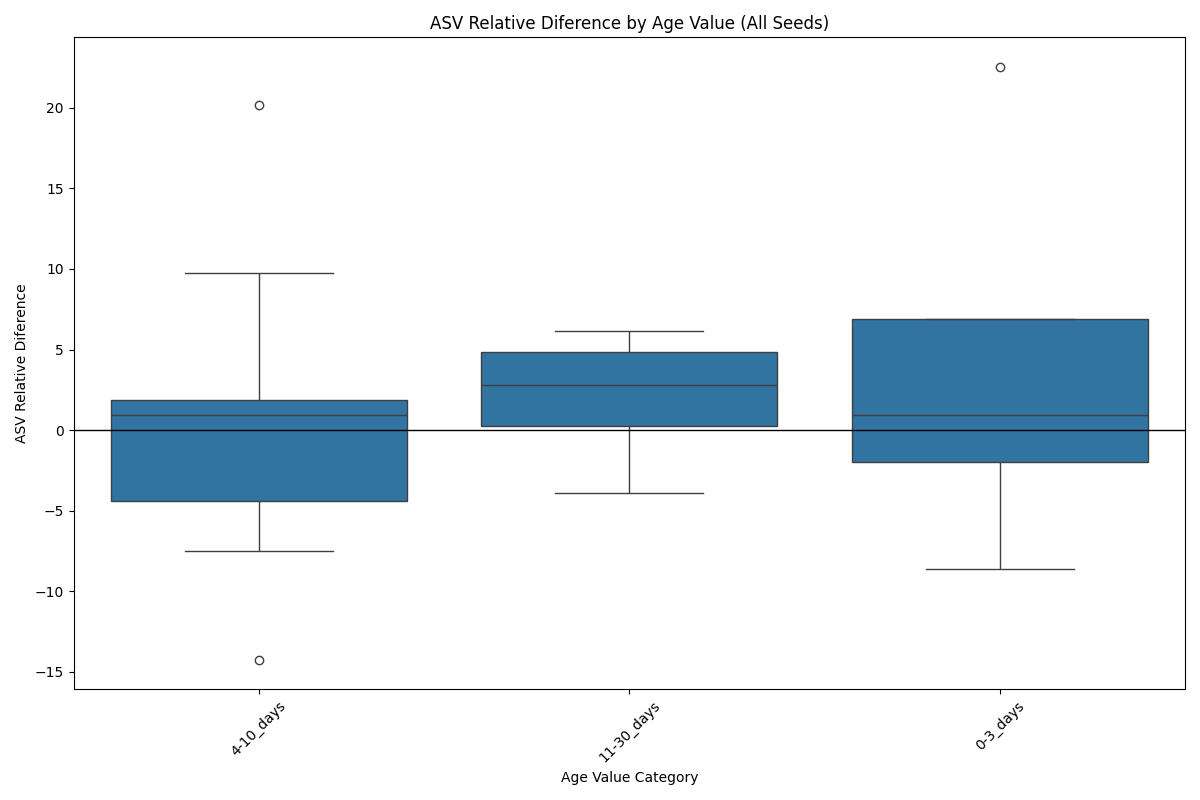
\includegraphics[width=0.8\linewidth]{img/asvResults/ChildAllSeedsASVBoxplot.png}
    \caption{Diferencia relativa entre los valores del ASV aproximado y el exacto para la red $\childNetwork$, se utilizaron las diferencias de cada una de las 5 seeds.}
    \label{fig:boxplotASVApproximateDifferences}
\end{figure}

% \echu{¿Tiene sentido hacer un experimento en el cuál comparo para distintos grafos, los árboles por ejemplo, cuán cercana es la distribución original a la sampleada? Puedo samplear y ver como me quedan distribuidas las clases de equivalencia. Intentando hacer algún calcúlo para ver cuán cercanas son esas clases de equivalencia a las originales. Respuesta de Santi: Noup, es justamente lo que hace el algoritmo, buscar samplear de las clases de equivalencia}

\subsection{Algoritmo de promedio para DT binarios}
\label{subSection:experimentoAlgoritmoPromedio}
Para este experimento vamos a comparar la forma naive de obtener la predicción promedio para una permutación y el algoritmo \ref{alg:meanPredBinDT}, que utiliza la estructura del árbol para calcularlo, con complejidad $O(i|V| + (varElim)l)$. La idea es comparar el tiempo que tardan ambos algoritmos y ver cómo se asemejan estos promedios a las probabilidades originales de la red. Dentro del cálculo de $\assym(x,i)$, para la instancia $x$ y el feature $i$, lo que queremos calcular es :
$$\charactheristicFunction(\toOr) = \mathbb{E}_{\aBayesianNetwork(x' | x)}[f_y(x_{\toOr \leq i} \cup x'_{\toOr > i})]$$

%\echu{La segunda es la fórmula que utilizo en la sección 2 para introducir al promedio, pero me gusta más la que utilizo acá porque siento que se entiende más para explicar la idea. ¿Puedo decir que ambas significan lo mismo y explicar porque? Además a M le falta el $_y$, aunque podría usar $M_y$ en vez de $f_y$ tal vez.}

A través de una permutación $\toOr$ de los features de $x$, definimos que features quedan fijos y cuales varían. La función de probabilidad que se utiliza es $\aBayesianNetwork(x' | x)$, la cual utilizamos para calcular la probabilidad de los valores de $x'$ dados los valores de $x$. Esta predicción promedio la vamos a calcular para cada uno de los posibles valores\footnote{Recordemos que podemos tener variables no binarias, por lo que $y$ puede tomar más valores que 0 o 1.} $y$ de $p$, el feature  a predecir.$f_y(x)$ es un clasificador binario, que devuelve $1$ si nuestro árbol de decisión le asigna la clase $y$ a la instancia $x$ y $0$ en el caso contrario. A continuación presentamos la implementación naive para calcular $\charactheristicFunction$. 
%\santi{El $y$ es el resultado entonces? ¿No alcanza entonces con poner $f_1()?$} Rta: No se había entendido que era para variables no binarias
%\echu{No entendí, $y$ es la clase que queres clasificar. Cómo no necesariamente son binarios los párametros entonces puede tomar todos los valores del dominio de la variable a predecir} 

Para calcular $\mathbb{E}_{\aBayesianNetwork(x' | x)}[f_y(x_{\toOr \leq i} \cup x'_{\toOr > i})]$ lo que vamos a hacer es: generar todas las instancias $x_{prom} \in (x_{\toOr \leq i} \cup x'_{\toOr > i})$, en las cuales los valores de los features que aparece luego de $x_i$ en $\toOr$ van a ser variables, y el resto van a ser fijos. Por fijos, nos referimos a que van tener los mismos valores que $x$, y sus otros features van a tomar todos los valores posibles. A partir de estas instancias vamos a calcular la función característica\footnote{La notación para la función característica es distinta a la utilizada al introducirla en la fórmula \ref{formula:characteristicFunctionDefinition}, pero su significado es el mismo. En este caso $(x_{\toOr \leq i} \cup x'_{\toOr > i})$ son nuestras instancias consistentes y $f_y$ es nuestro clasificador binario $M$. Para cada valor de $y$, $f_y$ devuelve 1 si la etiqueta clasificada es $y$ y 0 en el caso contrario.} cómo:

$$\charactheristicFunction(\toOr) = \sum_{x_{prom} \in (x_{\toOr \leq i} \cup x'_{\toOr > i})} p_\aBayesianNetwork(x_{prom} | x) f_y(x_{prom}) $$

%\santi{¿Para cuál valor de $y$?}
%\echu{Para cada valor de $y$ tenes una nueva función, lo aclare en el footnote. }

Por lo tanto, para esta cuenta vamos a necesitar generar todas las instancias $(x_{\toOr \leq i} \cup x'_{\toOr > i})$, y luego evaluar nuestro árbol de decisión $DT$ y a la red bayesiana $\aBayesianNetwork$ para cada una de estas instancias. Evaluar el $DT$ cuesta $O(d)$, siendo $d$ la profundidad del $DT$. Si tomamos a $c$ como la cardinalidad máxima de un feature y a $vars$ como el tamaño del conjunto de features variables, la complejidad temporal de la implementación naive es $O(vars^c(varElim + d)$, siendo $O(vars^c)$ la cantidad de instancias generadas. 

Así las complejidades que nos quedan son $O(vars^c(varElim + d))$ y $O(i|V| + (varElim)l)$, para cada uno de nuestros algoritmos. Podemos ver que la solución naive depende de la cantidad de features variables del $\toOr$, a diferencia del otro algoritmo, que corre el promedio directamente sobre la estructura del $DT$.

%\santi{$v$ no debería ser $|V|$? } Rta: Sip

%\echu{¿Tiene sentido lo de poner el valor que da la predicción del feature? Para mi un poco si para explicar que tipo de feature es y porque da esos valores. } Rta: Sip, tiene sentido

\begin{figure}[ht]
    \centering
    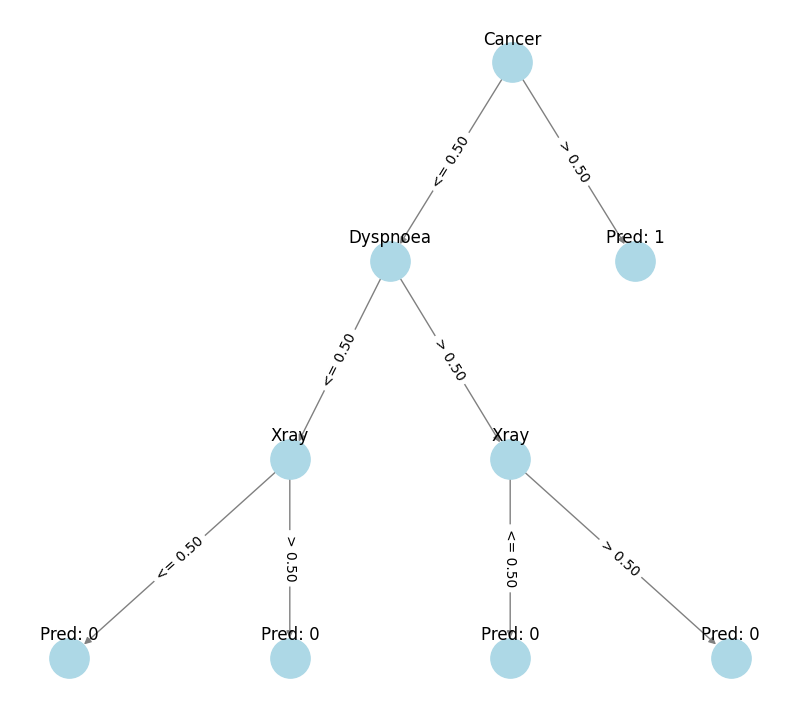
\includegraphics[width=0.7\linewidth]{img/cancerDecisionTree.png}
    \caption{Árbol de decisión generado a partir de los datos de la red $\cancerNetwork$, en las hojas está el valor de la predicción que devuelve el modelo (0 o 1)}
    \label{fig:cancerDecisionTree}
\end{figure}

Para la red $\cancerNetwork$ se generaron 600 instancias, con un árbol de decisión de altura 3 y para la red $\childNetwork$ se generaron 10000 instancias, con un árbol de decisión de altura 9. Las probabilidades de la red bayesiana son los valores que devuelve la consulta $P(X = z)$ para la red $\aBayesianNetwork$ y los distintos valores $z$ de cada feature $X$. El método \emph{Algoritmo promedio (probabilidades)}, consiste de la predicción promedio, si en el árbol en vez de devolver una predicción de 1 o 0, se devolviera una probabilidad en las hojas. Este método es distinto al algoritmo evaluado en esta tesis, pero nos pareció interesante agregarlo, para analizar la diferencia entre los promedios al usar una predicción probabilística. 
%\santi{Medio feo usar $y$ para dos cosas distintas.} Rta: Concuerdo

\begin{table}[ht]
    \centering
    \begin{tabular}{l c c}
        \toprule
        \textbf{M\'etodo} & \textbf{Predicci\'on} & \textbf{Tiempo (segundos)} \\
        \midrule
        Algoritmo promedio & [0.98255, 0.01745] & 0.0165 \\
        Algoritmo promedio (probabilidades) & [0.7213, 0.2787] & 0.0043 \\
        Implementaci\'on naive & [0.98255, 0.01745] & 0.0043 \\
        Probabilidades red bayesiana & [0.7, 0.3] & - \\
        \bottomrule
    \end{tabular}
    \caption{Valor promedio de la predicci\'on del feature \textbf{Smoker} en la red bayesiana $\cancerNetwork$, dejando variables todos los features}
    \label{table:cancerMeanResults}
\end{table}
%\sergio{Cuidado con la coherencia de CANCER, cancer, \it{cancer}} 

\begin{table}[ht]
    \centering
    \begin{tabular}{l c c}
        \toprule
        \textbf{M\'etodo} & \textbf{Predicci\'on} & \textbf{Tiempo (segundos)} \\
        \midrule
        Algoritmo promedio & [0.9916, 0.0, 0.0084] & 0.0258 \\
        Algoritmo promedio (probabilidades) & [0.7577, 0.0746, 0.1677] & 0.0258 \\
        Implementaci\'on naive & [0.9916, 0.0, 0.0084] & 19.6774 \\
        Probabilidades red bayesiana & [0.6490, 0.1715, 0.1795] & - \\
        \bottomrule
    \end{tabular}
    \caption{Valor promedio de la predicci\'on del feature \textbf{Age} en la red bayesiana $\childNetwork$, dejando variables 11 de los 20 features y utilizando a $x\in data$ t.q $f(x)=0$.}
    \label{table:childMeanResults}
\end{table}

Al analizar la Tabla \ref{table:cancerMeanResults} podemos ver que en ambos casos se tiende a sobrerrepresentar una clase. Esto ocurre ya que el modelo entrenado predice 0 para la mayoría de los inputs y la probabilidad de los inputs para los cuales predice 1 es más baja. En la Tabla \ref{table:childMeanResults} ocurre lo mismo respecto a la sobrerrepresentación. Por lo que, en realidad, la predicción promedio sólo va a ser tan buena como el modelo que haya sido entrenado, esto no depende del algoritmo, sino del entrenamiento del modelo.
Además, podemos ver que la implementación naive es más lenta, esto se debe a que la mediana de la cardinalidad de cada feature es 3. Por lo que cada feature agregado va a hacer que se tarde 3 veces más en promedio, para órdenes topológicos que dejaran los 19 features variables la implementación naive tardaría \textbf{más de 1 día}. En cambio, la performance del algoritmo promedio no se ve tan afectada por la cantidad de features variables, sino que depende del tamaño del árbol de decisión. Finalmente, se destaca que las predicciones más cercanas a las probabilidades generadas por la red bayesiana son aquellas que utilizan directamente las probabilidades como output, en lugar de predicciones binarias (0/1). Esto se debe a que estas predicciones son más granulares y, por ende, reflejan con mayor fidelidad las distribuciones probabilísticas subyacentes.

Se puede contemplar que los valores de la implementación naive y del algoritmo promedio son idénticos, puesto que ambos están calculando lo mismo. Sólo que mientras nuestro algoritmo calcula la probabilidad de llegar a una hoja, la implementación naive genera todas las instancias que pueden llegar a la misma, para luego clasificarlas y calcular su probabilidad. 
%Esto ocurre ya que el algoritmo del promedio en $DT$ utiliza las hojas del $DT$ para realizar su cálculo, en cambio, la implementación naive genera instancias nuevas a partir de los features variables. Por lo que no necesariamente van a tener el mismo valor estos dos algoritmos, aun así su diferencia no va a ser significativa. Esto puede significar un problema para nuestro algoritmo si resulta que el árbol de decisión no tiene instancias representativas en sus hojas, ya que el valor del promedio no va a tener en cuenta a una muestra significativa. 
%\sergio{Revisar, repensar, repent. No deberia dar distinto, revisar el caso en el cual da y evaluar porque. Si es que no es un bug y tiene sentido, meteer una oraci[on que lo explique mejor. } RTA: Había flasheado, al final si eran iguales
%\santi{Adem[as en la seccion hablas del valor de la prediccion ylos comparas. Cuando en la intro solo hablas del tiempo, aclarar que se va a tener eso en cuenta tambi[en. Si no lo vas a hacer, remover el valor de las tablas.}

Podemos ver en la Figura~\ref{fig:cancerDecisionTree} que el patrón aprendido por el árbol es muy simple $f(x) = $ \textbf{If} $x_{cancer} > 0.5$, \textbf{then} 1, \textbf{else} 0. Luego como $P(Cancer = 1) = 0.01745$, por lo que el promedio que vemos en la Tabla \ref{table:cancerMeanResults} va a representar esa predicción. 

%\santi{Mover esta primer expeimentación al final, es la menos importante.}

%\sergio{recordar de unificar capitalización Tablas, Sección, Figura, etc.}